\chapter{Desarrollo. Entregas e iteraciones}
\label{ch:desarrollo}
Este capítulo recoge el proceso de desarrollo del juego, en el que se detallan las diferentes entregas e iteraciones, así como los resultados de estas.

\section{Entrega 0}

\subsection{Primera iteración}

\section{Entrega 1}
En esta entrega se han llevado a cabo bocetos del juego, y pruebas heurísticas y de usuario sobre estos.

%%%%%%%%%%%%%%%%%%%%%%%%%%%%%%%%%%%%%%%%%%%%%%%%%% BOCETOS %%%%%%%%%%%%%%%%%%%%%%%%%%%%%%%%%%%%%%%%%%%%%%%%%%%%%%
\subsection{Bocetos}
Se han creado bocetos que representan la idea inicial del juego y cómo serán sus diferentes pantallas e interfaces, de forma que se puedan utilizar para llevar a cabo pruebas sobre ellos, dichas pruebas incluyen pruebas heurísticas realizadas por el desarrollador y pruebas se usabilidad con usuarios reales, para así saber que esta bien y que no en los bocetos y mejorar el diseño del juego.\\

En la Figura \ref{figura-b1} se puede ver el boceto creado para la pantalla inicial en la que se seleccionará los personajes con los que se quiere jugar:

\begin{figure}[h]
  \centering
  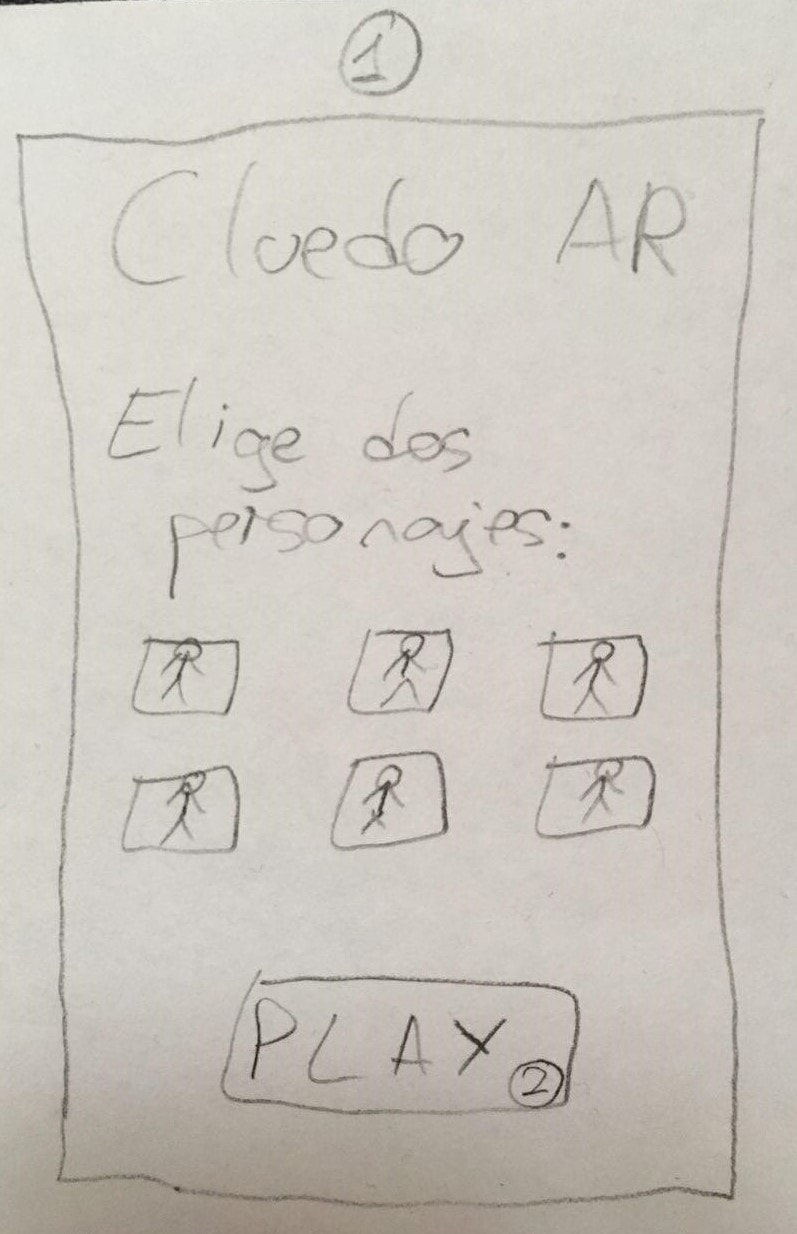
\includegraphics[scale=0.2]{b1}
  \caption{Imagen que muestra la interfaz de la pantalla inicial del juego.\protect\footnotemark}
  \label{figura-b1}
\end{figure}

\newpage

En la Figura \ref{figura-b2} se puede ver el boceto creado para la pantalla de instrucciones:

\begin{figure}[h]
  \centering
  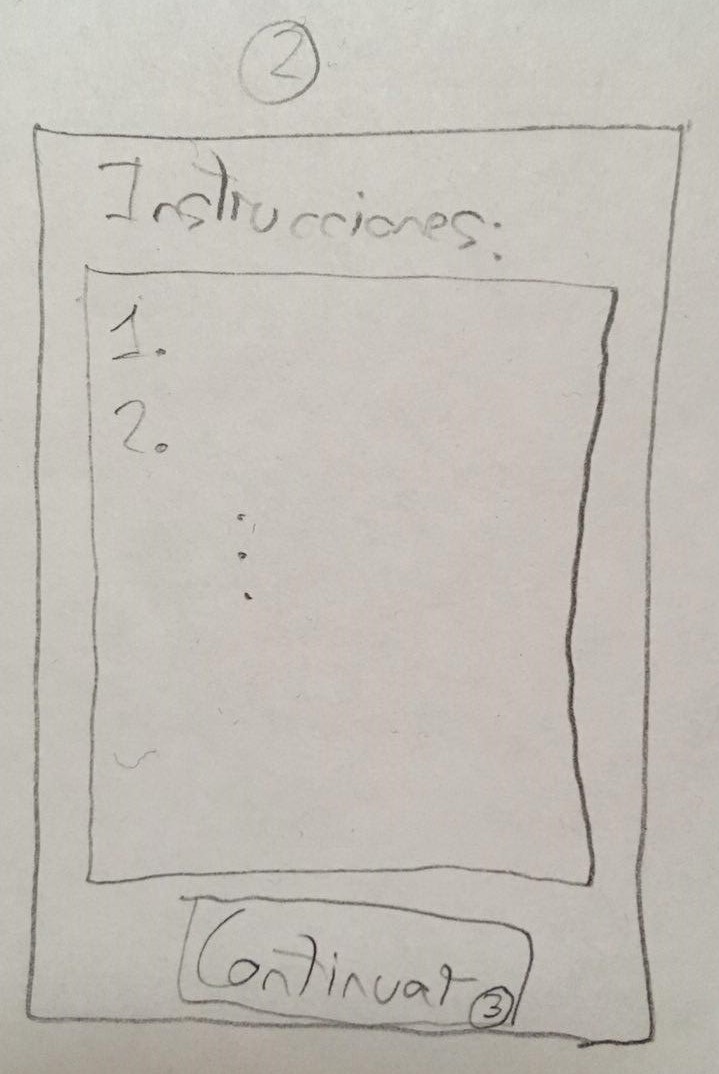
\includegraphics[scale=0.2]{b2}
  \caption{Imagen que muestra la interfaz de la pantalla de instrucciones del juego.\protect\footnotemark}
  \label{figura-b2}
\end{figure}

El resto de los bocetos se pueden encontrar en la sección \ref{bocetos} del Anexo.

\subsection{Pruebas heurísticas}
\begin{itemize}

  \item \textbf{Principio 1: Visibilidad del estado del sistema.}\\
  La puntuación es de 7, el usuario está bien informado de lo que ocurre actualmente en el sistema, se muestra siempre que es necesario el botón “home” o el botón “atrás”, pero se puede mejorar, por ejemplo, indicando que se están escaneando imágenes mientras mueves el dispositivo sobre el tablero.

  \item \textbf{Principio 2: Correspondencia entre el sistema y el mundo real.}\\
  La puntuación es de 10, las opciones en los menús están ordenadas de forma lógica y el lenguaje que el juego utiliza es un lenguaje común al usuario del juego.

  \item \textbf{Principio 3: Control y libertad del usuario.}\\
  La puntuación es de 7, ya que en la mayoría de pantallas el usuario es libre de ir hacia adelante o hacia atrás, pero en instrucciones el usuario puede avanzar al juego pero no volver a la pantalla de inicio. Además, como se puede ver en la pantalla 6, para hacer apuntes, el botón de retroceso está en la zona derecha de la pantalla, pudiendo confundir esto al usuario, ya que es una función de retroceso no de avance.

  \item \textbf{Principio 4: Consistencia y estándares.}\\
  La puntuación es de 7, ya que es bastante consistente, pero en la pantalla que indica el ganador aparece el botón “home” como en otras pantallas, pero se muestra en una posición distinta, lo que resulta confuso al usuario habría que moverlo a la posición que ocupa siempre o utilizar otro botón.

  \item \textbf{Principio 5: Prevención de errores.}\\
  La puntuación es de 10, el diseño es bastante cuidadoso para la prevención de errores y el correcto tratamiento de estos.

  \item \textbf{Principio 6: Minimizar la carga de memoria del usuario.}\\
  La puntuación es de 10, el usuario no necesita recordar nada en ningún momento, todo se muestra de forma apropiada para que no suponga ninguna memorización al usuario.

  \item \textbf{Principio 7: Personalización y atajos.}
  La puntuación es de 10, la aplicación no dispone de personalización o atajos, pero no son necesarios en esta, por lo que no afecta a la experiencia de usuario.

  \item \textbf{Principio 8: Eficiencia de uso y rendimiento.}
  La puntuación es de 8, la aplicación está bien optimizada para que al usuario le resulte sencillo y rápido llevar a cabo cualquier tarea, pero si es cierto que algunos botones que se utilizan con mucha frecuencia no están en las posiciones óptimas.

  \item \textbf{Principio 9: Estética y diseño minimalista.}
  La puntuación es de 10, la información que se muestra en la aplicación es la necesaria para que el usuario pueda jugar con la mejor experiencia de usuario posible, no hay exceso o falta de información.

  \item \textbf{Principio 10: Ayuda al usuario a reconocer, diagnosticar y recuperarse de errores.}
  La puntuación es de 10, ya que no hay posibilidad de que ocurran errores en el juego.

  \item \textbf{Principio 11: Ayuda y documentación.}
  La puntuación es de 10, ya que antes de comenzar cada partida se muestra al usuario unas instrucciones de cómo funciona el juego.

  \item \textbf{Principio 12: Interacción física y ergonomía.}
  La puntuación es de 10, ya que los botones son fácilmente diferenciables y están en una posición cómoda para el usuario, teniendo en cuenta que al ser un juego utilizará las dos manos para usar el dispositivo móvil.

\end{itemize}

\subsection{Pruebas de usabilidad}
Las tablas que contienen la información obtenida en estas pruebas de usabilidad se encuentran en la sección \ref{tablas-usabilidad-bocetos} del Anexo.

\begin{itemize}
  \item \textbf{Usuario 1}

  \textbf{Pre Test}

  \begin{enumerate}
    \item Edad: 18
    \item Dispone de un dispositivo móvil: Sí
    \item Con qué frecuencia utiliza su dispositivo móvil: Varias veces al dia
    \item Con qué frecuencia juega a juegos de mesa: Varias veces al año
    \item Con qué frecuencia juega a juegos en su móvil: Varias veces a la semana
  \end{enumerate}

  \textbf{Test}: Los resultados del test de usabilidad sobre el Usuario 1 se encuentran en la Tabla \ref{tabla-bocetos-usuario1}


  \item \textbf{Usuario 2}

  \textbf{Pre Test}

  \begin{enumerate}
    \item Edad: 57
    \item Dispone de un dispositivo móvil: Sí
    \item Con qué frecuencia utiliza su dispositivo móvil: Varias veces al día
    \item Con qué frecuencia juega a juegos de mesa: Varias veces al año
    \item Con qué frecuencia juega a juegos en su móvil: Varias veces al día
  \end{enumerate}

  \textbf{Test}: Los resultados del test de usabilidad sobre el Usuario 2 se encuentran en la Tabla \ref{tabla-bocetos-usuario2}


  \item \textbf{Usuario 3}

  \textbf{Pre Test}

  \begin{enumerate}
    \item Edad: 26
    \item Dispone de un dispositivo móvil: Sí
    \item Con qué frecuencia utiliza su dispositivo móvil: Varias veces al dia
    \item Con qué frecuencia juega a juegos de mesa: Una vez al mes como máximo
    \item Con qué frecuencia juega a juegos en su móvil: Casi nunca
  \end{enumerate}

  \textbf{Test}: Los resultados del test de usabilidad sobre el Usuario 3 se encuentran en la Tabla \ref{tabla-bocetos-usuario3}

\subsection{Segunda iteración}

\subsection{Conclusiones}
Durante dichas pruebas hemos podido comprobar que la interfaz de la aplicación es amigable para los usuarios, que si bien han detectado algunos fallos, que serán solventados en el desarrollo del juego, por lo general han sabido realizar todas las tareas sin dificultad, desenvolviéndose con rapidez.\\

También se ha podido comprobar el interés de los usuarios por el funcionamiento de la realidad aumentada, resultándoles algo sorprendente y que sin duda tenían ganas de probar en las siguientes pruebas de usabilidad, lo que denota la esperada expectación de los usuarios de juegos y en general de dispositivos móviles sobre la realidad aumentada y las novedosas experiencias que esta aportará al ámbito de los dispositivos móviles.

\section{Entrega 2}

\subsection{Tercera iteración}

\subsection{Cuarta iteración}

\section{Entrega 3}

\subsection{Quinta iteración}

\subsection{Sexta iteración}

\subsection{Séptima iteración}

\section{Entrega 4}

\subsection{Octava iteración}
